\section{Softwarearchitektur (8P)}

\subsection{Gewählte Architektur (4P)}
\task{In der Vorlesung wurden Softwarearchitekturen vorgestellt. Welche Architektur wurde davon umgesetzt? Analyse und Begründung inkl. UML der wichtigsten Klassen, sowie Einordnung dieser Klassen in die gewählte Architektur}
Das Projekt basiert auf einem Schichtenmodel, wobei die Main Klasse als Präsentationschicht dient, die Commands und der CommandController als Domänenschicht und die SQL-Klassen als Datenschicht.  
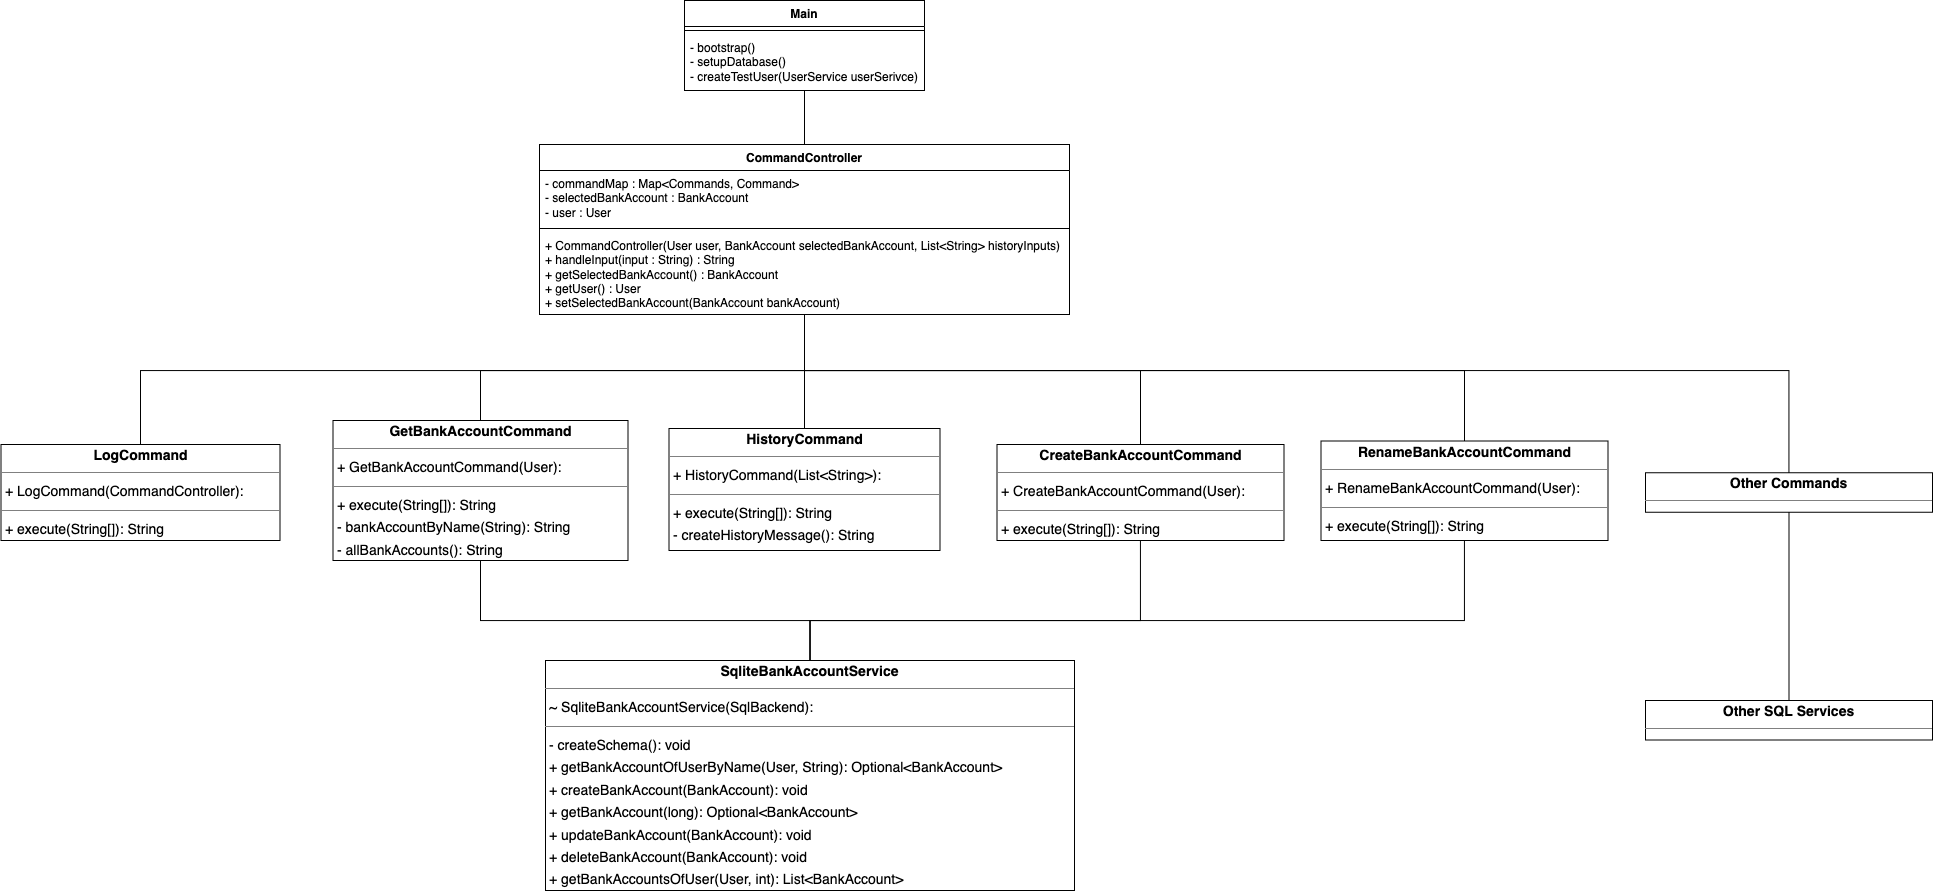
\includegraphics[width=\linewidth]{kapitel2_architektur/Softwarearchitekturen.drawio.png}
\subsection{Domain Code (1P)}
\task{kurze Erläuterung in eigenen Worten, was Domain Code ist – 1 Beispiel im Code zeigen, das bisher noch nicht gezeigt wurde}
Domain Code bezeichnet den Code, der die Geschäftslogik einer Anwendung enthält. Er beschreibt die Kernlogik eines Systems und bildet die Fachdomäne (Domain) des Unternehmens oder Projekts ab. 
\lstinputlisting[language=Java,style=codeStyle]{kapitel2_architektur/ddd1.java}
\subsection{Analyse der Dependency Rule (3P)}
\task{In der Vorlesung wurde im Rahmen der ‘Clean Architecture’ die s.g. Dependency Rule vorgestellt. Je 1 Klasse zeigen, die die Dependency Rule einhält und 1 Klasse, die die Dependency Rule verletzt;   jeweils UML (mind. die betreffende Klasse inkl. der Klassen, die von ihr abhängen bzw. von der sie abhängt) und Analyse der Abhängigkeiten in beide Richtungen (d.h., von wem hängt die Klasse ab und wer hängt von der Klasse ab) in Bezug auf die Dependency Rule}
\subsubsection*{Positiv-Beispiel: Dependency Rule}
\subsubsection*{Negativ-Beispiel: Dependency Rule}